\documentclass[journal,12pt,twocolumn]{IEEEtran}

\usepackage{setspace}
\usepackage{gensymb}
\singlespacing
\usepackage[cmex10]{amsmath}

\usepackage{amsthm}

\usepackage{mathrsfs}
\usepackage{txfonts}
\usepackage{stfloats}
\usepackage{bm}
\usepackage{cite}
\usepackage{cases}
\usepackage{subfig}

\usepackage{longtable}
\usepackage{multirow}

\usepackage{enumitem}
\usepackage{mathtools}
\usepackage{steinmetz}
\usepackage{tikz}
\usepackage{circuitikz}
\usepackage{verbatim}
\usepackage{tfrupee}
\usepackage[breaklinks=true]{hyperref}
\usepackage{graphicx}
\usepackage{tkz-euclide}

\usetikzlibrary{calc,math}
\usepackage{listings}
    \usepackage{color}                                            %%
    \usepackage{array}                                            %%
    \usepackage{longtable}                                        %%
    \usepackage{calc}                                             %%
    \usepackage{multirow}                                         %%
    \usepackage{hhline}                                           %%
    \usepackage{ifthen}                                           %%
    \usepackage{lscape}     
\usepackage{multicol}
\usepackage{chngcntr}

\DeclareMathOperator*{\Res}{Res}

\renewcommand\thesection{\arabic{section}}
\renewcommand\thesubsection{\thesection.\arabic{subsection}}
\renewcommand\thesubsubsection{\thesubsection.\arabic{subsubsection}}

\renewcommand\thesectiondis{\arabic{section}}
\renewcommand\thesubsectiondis{\thesectiondis.\arabic{subsection}}
\renewcommand\thesubsubsectiondis{\thesubsectiondis.\arabic{sub subsection}}


\hyphenation{optical networks semiconduc-tor}
\def\inputGnumericTable{}                                 %%

\lstset{
%language=C,
frame=single, 
breaklines=true,
columns=fullflexible
}
\date{March 2021}

\begin{document}

\newcommand{\BEQA}{\begin{eqnarray}}
\newcommand{\EEQA}{\end{eqnarray}}
\newcommand{\define}{\stackrel{\triangle}{=}}
\bibliographystyle{IEEEtran}
\raggedbottom
\setlength{\parindent}{0pt}
\providecommand{\mbf}{\mathbf}
\providecommand{\pr}[1]{\ensuremath{\Pr\left(#1\right)}}
\providecommand{\qfunc}[1]{\ensuremath{Q\left(#1\right)}}
\providecommand{\fn}[1]{\ensuremath{f\left(#1\right)}}
\providecommand{\e}[1]{\ensuremath{E\left(#1\right)}}
\providecommand{\sbrak}[1]{\ensuremath{{}\left[#1\right]}}
\providecommand{\lsbrak}[1]{\ensuremath{{}\left[#1\right.}}
\providecommand{\rsbrak}[1]{\ensuremath{{}\left.#1\right]}}
\providecommand{\brak}[1]{\ensuremath{\left(#1\right)}}
\providecommand{\lbrak}[1]{\ensuremath{\left(#1\right.}}
\providecommand{\rbrak}[1]{\ensuremath{\left.#1\right)}}
\providecommand{\cbrak}[1]{\ensuremath{\left\{#1\right\}}}
\providecommand{\lcbrak}[1]{\ensuremath{\left\{#1\right.}}
\providecommand{\rcbrak}[1]{\ensuremath{\left.#1\right\}}}
\theoremstyle{remark}
\newtheorem{rem}{Remark}
\newcommand{\sgn}{\mathop{\mathrm{sgn}}}
\providecommand{\abs}[1]{\vert#1\vert}
\providecommand{\res}[1]{\Res\displaylimits_{#1}} 
\providecommand{\norm}[1]{\lVert#1\rVert}
%\providecommand{\norm}[1]{\lVert#1\rVert}
\providecommand{\mtx}[1]{\mathbf{#1}}
\providecommand{\mean}[1]{E[ #1 ]}
\providecommand{\fourier}{\overset{\mathcal{F}}{ \rightleftharpoons}}
%\providecommand{\hilbert}{\overset{\mathcal{H}}{ \rightleftharpoons}}
\providecommand{\system}{\overset{\mathcal{H}}{ \longleftrightarrow}}
	%\newcommand{\solution}[2]{\textbf{Solution:}{#1}}
\newcommand{\solution}{\noindent \textbf{Solution: }}
\newcommand{\cosec}{\,\text{cosec}\,}
\providecommand{\dec}[2]{\ensuremath{\overset{#1}{\underset{#2}{\gtrless}}}}
\newcommand{\myvec}[1]{\ensuremath{\begin{pmatrix}#1\end{pmatrix}}}
\newcommand{\mydet}[1]{\ensuremath{\begin{vmatrix}#1\end{vmatrix}}}
\numberwithin{equation}{subsection}
\makeatletter
\vspace{3cm}
\title{ASSIGNMENT 9}
\author{MANIKANTA VALLEPU - AI20BTECH11014}
\maketitle
\newpage
\bigskip
\renewcommand{\thetable}{\theenumi}
Download all python codes from 
\begin{lstlisting}
https://github.com/manik2255/AI1103-PROBABILITY-AND-RANDOM-VARIABLES/blob/main/ASSIGNMENT_9/assign_9.py
\end{lstlisting}
%
and latex-tikz codes from 
%
\begin{lstlisting}
https://github.com/manik2255/AI1103-PROBABILITY-AND-RANDOM-VARIABLES/blob/main/ASSIGNMENT_9/ASSIGNMENT_9.tex
\end{lstlisting}
\section{GATE 2021 (ME-SET1)PROBLEM.33}
Customers arrive at a shop according to Poisson distribution with a mean of 10 customers/hour. The manager notes that no customer arrives for the first 3 minutes after the shop opens. The probability that a customer arrives within the next 3 minutes is
\section{solution}
Given, 
mean of 10 customers arrive in a time interval of 60 minutes $\iff$ mean of $\dfrac{t}{6}$ customers arrive in a time interval of t minutes,
Customers arrive according to Poisson distribution with a mean of $\dfrac{t}{6}$ customers/t minutes,
\begin{align}
\therefore \lambda = \frac{t}{6} \label{a}
\end{align}
Let $X$ denotes the number of customers in first t minutes,$Y$ denotes the number of customers in second t minutes.
according to  poisson distribution,
\begin{align}
\pr{X=x}= e^{-\lambda} \frac{\lambda^{x}}{x\,!} \label{b}
\end{align}
using \eqref{a} in \eqref{b},
\begin{align}
\pr{X=x}= e^{-\frac{t}{6}} \frac{(\frac{t}{6})^{x}}{x\,!} \label{c}
\end{align}
 the probability that a customer arrives within the next t minutes given that no customer arrives for the first t minutes after the shop opens,which can also be written as,
\begin{align}
\pr{Y\neq 0|X=0}=\frac{\pr{Y\neq 0,X=0}}{\pr{X=0}}
\end{align}
\begin{table}[ht]
\caption{Probability distribution for values of X and Y}
\begin{center}
    \begin{tabular}{|c|c|c|}
    \hline
     & P(X)&P(Y)\\
    \hline
    0& $e^{-\frac{t}{6}}$& $e^{-\frac{t}{6}}$\\
    \hline
    1 & $\frac{t e^{-\frac{t}{6}}}{6}$ & $\frac{t e^{-\frac{t}{6}}}{6}$\\
    \hline
    \end{tabular}
\end{center} 
\end{table}

As the arrival of customers in second t minutes does not depend on the arrival of customers in first t minutes, X and Y are independent,
\begin{align}
\pr{Y\neq 0|X=0}&=\frac{\pr{Y\neq 0}\pr{X=0}}{\pr{X=0}}\\
&=\pr{Y\neq 0}\\
&= 1-\pr{Y=0} 
\end{align}
using \eqref{c},
\begin{align}
\pr{Y\neq 0|X=0}&=1- e^{-\frac{t}{6}}
\end{align}
we need to find the probability for t=3,the required probability is given by,
\begin{align}
&=1- e^{-\frac{1}{2}}\\
&=0.3935
\end{align}
\begin{figure}[ht]
    \centering
    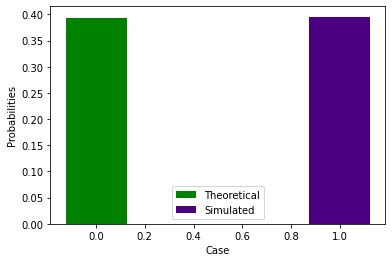
\includegraphics[width=\columnwidth]{assign_9.png}
    \caption{Theoretical vs simulation}
\label{fig_1}
\end{figure}
\end{document}

